\part{Hybridné modelovanie a jeho využitie v praxi}
\chapter{Hybridné modelovanie}
Úlohou modelovania procesov je získať matematický predpis na základe znalostí, ktoré o tomto procese máme \cite{hangos:process_modelling:2001}. V závislosti od prístupu k modelovaniu, môžeme získané modely rozdeliť do viacerých skupín. Prvou skupinou sú tak zvané \aps{mechanické} modely. Tieto sú odvodené z fyzikálnych zákonov, ktoré predstavujú rôzne zákony zachovania -- bilancie, hmoty alebo energie, zákony kinetiky, termodynamiky, prestupu látky atď \cite{bangi:chem_engineer:2020}. Takéto modely sú transparentné a ľahko pochopiteľné, pretože majú za sebou skutočnú fyzikálnu podstatu, ktorá platí pre široké spektrum operačných podmienok. Nevýhodou býva, že často sú veľmi zložité a samotné modelovanie je náročné na čas. Druhú skupinu tvoria dátové modely, ktorých problematiku sme rozobrali v predchádzajúcich kapitolách. Spomenieme, že majú viacero výhod -- sú jednoduché na získanie, čím ušetríme kopec času s modelovaním, často majú jednoduchšiu štruktúru, sú flexibilnejšie atď. Nevýhodou však je, že ich štruktúra nám neprezradí nič o samotnej povahe procesu. Hybridné modely tvoria tretiu skupinu a  sú kombináciou mechanických a dátových modelov, pričom využívajú výhody z obidvoch skupín, čím našli široké uplatnenie v rôznych oblastiach -- bioinžinierstvo \cite{srivastava:hybrid_biomolecules:2020}, strojníctvo \cite{liu:hybrid_vehicle:2020}, životné prostredie \cite{liu:hybrid_waste_water:2019}, energetika \cite{qian:hybrid_energy:2019} atď.

\section{Hybridné modely}
Základy hybridného modelovania položili Psichogios a Ungar v práci \aps{\textit{A hybrid neural network-first principles approach to process modeling}} z roku 1992 \cite{psichogios:hybrid_process_model:1992}. Ich cieľom bolo vytvoriť hybridný model založený na neurónovej sieti a mechanickom modely vsádzkového biochemického reaktora. Vo výsledku sa im podarilo zlepšiť presnosť predikcie v porovnaní so samotným mechanickým modelom, dosiahnuť lepšiu interpoláciu a extrapoláciu na rozdiel od samotnej neurónovej sieti a výrazne sa uľahčila analýza a interpretácia dát.

Existuje veľa rôznych kombinácii mechanických a dátových modelov, ktoré vedú k ešte väčšiemu množstvu hybridných modelov, ale vo všeobecnosti by sme mohli takýto model sformulovať nasledovne
\begin{equation}
	\begin{split}
		\der{x}{t} &= f(t,x,u,\theta), \\
		\theta &= g(x,u),
	\end{split}
\end{equation}
kde $ x $ predstavuje stavy, $ u $ vstupy, $ \theta $ parametre procesu. Celá dynamika systému je definovaná funkciou $ f $, ktorá predstavuje základný mechanický model a je závislá na parametroch systému $ \theta $, ale tie zasa závisia od stavov $ x $ a vstupov $ u $, ktoré vieme získať z dátovej časti. Takáto štruktúra hybridného modelu je zobrazená aj na Obr. \ref{fig:hybrid_model_general}.

\begin{figure}
	\centering
	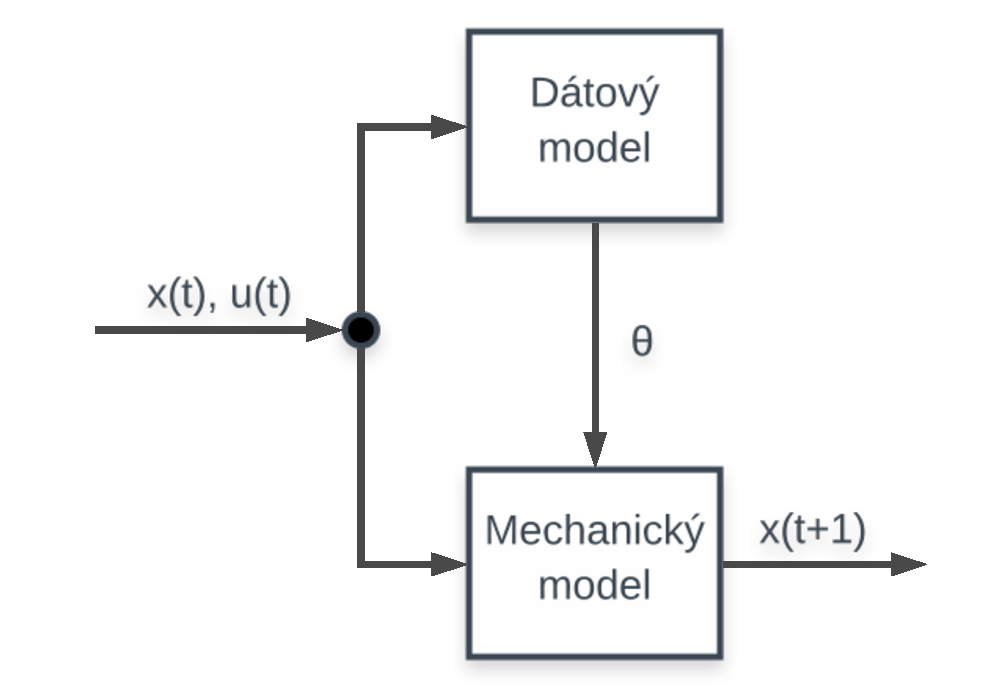
\includegraphics[width=0.5\linewidth]{images/hybrid_model}
	\caption{Príklad všeobecného hybridného modelu.}
	\label{fig:hybrid_model_general}
\end{figure}

Treba zdôrazniť, že pri viacerých chemických, biologických a rôznych ďalších procesoch sú parametre modelu neznáme, pretože zohľadňujú napr. kinetiku konkrétnej chemickej reakcie alebo rast mikroorganizmov, ktorý je špecifický pre konkrétny druh. Ak dátový model dokáže poskytnúť tieto neznáme parametre mechanickému modelu, tak výsledný hybridný model je vhodný aj na predikciu údajov, a tým pádom sa môže využiť na optimalizáciu procesov. 